\documentclass[conference]{IEEEtran}
\IEEEoverridecommandlockouts
% The preceding line is only needed to identify funding in the first footnote. If that is unneeded, please comment it out.
\usepackage{cite}
\usepackage{amsmath,amssymb,amsfonts}
\usepackage{algorithmic}
\usepackage{graphicx}
\usepackage{textcomp}
\usepackage{xcolor}
\usepackage{CJK}
\usepackage{CJKutf8}
\usepackage{booktabs}

\def\BibTeX{{\rm B\kern-.05em{\sc i\kern-.025em b}\kern-.08em
    T\kern-.1667em\lower.7ex\hbox{E}\kern-.125emX}}
\begin{document}
\begin{CJK*}{UTF8}{gbsn}%{bsmi}

\title{LLM-OCR-SWPC: Hanzi’s Cognitive Advantage and Token Efficiency in Multimodal AI\\

\thanks{This work has been partially supported by the Brazilian National Council for Scientific and Technological Development (CNPq).}
}

\author{\IEEEauthorblockN{Li Weigang}
\IEEEauthorblockA{\textit{TransLab, Computer Science Department} \\
\textit{University of  Brasilia, Brasília, Brazil}\\
weigang@unb.br}
\and

\IEEEauthorblockN{João Paulo Vieira Costa}
\IEEEauthorblockA{\textit{TransLab, Computer Science Department} \\
\textit{University of  Brasilia, Brasília, Brazil}\\
jpcosta1990@gmail.com}


}


\maketitle

\begin{abstract}
With the rapid progress of vision–language models such as DeepSeek-OCR and CogVLM, the properties of writing systems in multimodal tokenization have become increasingly important. Based on the Six-Writings Pictophonetic Coding (SWPC) principle, this paper proposes LLM-OCR-SWPC, a Hanzi-centered multimodal framework that jointly encodes graphical structure, phonetic features, and semantic grounding within a single cognitive representation. Unlike phonetic scripts such as Japanese Kana, which distribute meaning across multiple characters, Hanzi embeds compositional semantics inside each glyph, enabling more efficient visual–semantic coupling. Using a multilingual chemical terminology dataset, we evaluate Average Byte Length, Visual Token Density, Semantic Decoding Accuracy, and entropy shift |ΔH|/d. Results show that Hanzi achieves up to 2–5× higher multimodal token efficiency and significantly lower entropy variation than Kana and English, providing quantitative evidence for its cognitive advantage in visual LLM encoding. LLM-OCR-SWPC reframes Chinese NLP as symbolic–cognitive modeling and offers a theoretically grounded complement to current LLM-OCR architectures. These findings suggest that Hanzi is not only a linguistic script but a computationally efficient symbolic system whose internal structure can be directly exploited by multimodal LLMs.
\end{abstract}

%With the rapid improvement of visual capabilities in LLMs, systems such as DeepSeek-OCR and CogVLM have demonstrated strong performance in image understanding. Building on the Six-Writings Pictophonetic Coding (SWPC) theory, this paper proposes a new Hanzi visual processing framework—LLM-OCR-SWPC—which integrates graphical, phonetic, and semantic information within visual embeddings, enabling “once-learning” cognitive behavior and improving visual processing efficiency.
%Unlike phonetic scripts such as Japanese Kana, which lack internal structure, Hanzi characters encode interpretable form and composition inside a single glyph. This leads to stronger visual–semantic coupling in OCR-based multimodal reasoning. Using a cross-lingual dataset of chemical element terms (e.g., “氢–H–Hydrogen”), to evaluate visual token density, byte-length efficiency, and semantic recovery accuracy, the results show that, under comparable image compression settings, Hanzi can achieve up to 97\% decoding accuracy with fewer visual tokens and lower entropy fluctuations than Kana.
%This study reframes Chinese NLP from a purely data-driven engineering problem into a symbolic-cognitive modeling discipline. LLM-OCR-SWPC provides a theoretical cognitive foundation for multimodal AI and offers a complementary and extensible development path for existing LLM-OCR architectures.


\begin{IEEEkeywords}
Chinese Hanzi, CNLP, DeepSeek-OCR, multimodal processing, LLM, Once learning, Six-Writings principle
\end{IEEEkeywords}

\section{Introduction}
The development of multimodal large language models (LLMs) such as DeepSeek-OCR \cite{wei2025deepseek} and Tsinghua-VLM \cite{wang2024cogvlm} has revitalized research on cross-domain perception and linguistic integration. These systems, originally designed for visual recognition, have achieved remarkable decoding precision—DeepSeek-OCR, for instance, attains 97\% accuracy when the number of text tokens remains within ten times that of vision tokens (compression ratio $<$ 10×) \cite{wei2025deepseek}. CogVLM's visual expertise complements DeepSeek-OCR by enabling semantic reasoning on decoded Hanzi. Yet, such progress primarily concerns the \textit{recognition} of characters rather than their deeper \textit{understanding} in the context of cognitive and linguistic structures.

Hanzi presents a unique cognitive system that combines pictorial, phonetic, and semantic information within a single symbol. Historically, this high information density has repeatedly influenced technological transitions—from the invention of efficient Chinese typewriters in the 1910s–1930s, where radical-based layouts eventually surpassed the typing speed of alphabetic keyboards \cite{mullaney2017chinese,weigang2022typewriter}, to Wang Xuan’s contour–parameter laser photo-composition system for Hanzi printing in the 1980s \cite{wangxuan1997}, which revolutionized digital typography. During the information revolution, coding systems such as Cangjie and Wubi further enabled Hanzi to coexist with computers through structure-based decomposition, thereby preserving linguistic autonomy despite the dominance of alphabetic scripts \cite{sun2021chinesebert,weigang2025threshold}.  A fundamental theoretical basis is provided by Six-Writings Pictophonetic Coding (SWPC) \cite{weigang2024six}, which enables LLMs to model the internal structural, phonetic, and semantic properties of Hanzi in Chinese natural language processing (CNLP). Building on this foundation, the present work extends SWPC to visual processing through LLM-OCR-SWPC.

In the current era of artificial intelligence, language models remain predominantly English-centric. Most multilingual LLMs handle non-English inputs through implicit English pivots (EN$\leftrightarrow$ZH translations), achieving fluent but sometimes semantically unstable outputs. Such token-level transformations overlook the visual and structural compactness of Hanzi, where a single character (≈3 bytes in UTF-8) often encodes what requires multiple tokens in other languages—Japanese, for instance, averages 4.58 characters and 13.73 bytes per conceptual unit in periodic table of chemical elements.

Motivated by these observations, this work investigates whether Hanzi’s picto-semantic structure can yield measurable advantages in visual–semantic efficiency under OCR-style encoding. We hypothesize that when visual models process textual information directly from character images, the inherent compression of Hanzi enables higher semantic recoverability with fewer vision tokens. In other words, \textbf{Hanzi may serve as an optimal visual-semantic encoding language for multimodal LLMs}.

To test this hypothesis, LLM-OCR-SWPC is used to perform a small-scale comparative study between Chinese and Japanese representations of scientific entities (e.g., chemical elements). Using an OCR-style encoding and decoding pipeline inspired by DeepSeek-OCR, we quantify (i) compression ratio, (ii) decoding precision, and (iii) semantic recoverability. The results show that Hanzi consistently achieves high decoding accuracy (≈97\%) at lower token densities, supporting the notion that Hanzi possesses intrinsic multimodal efficiency for AI-driven cognition.

This study aims to bridge modern OCR-based vision–language modeling, LLM-OCR-SWPC, with the long-standing cognitive theory of \textit{Once-Learning} \cite{weigang1999study,weigang2022hol,althoff2022once} and SWPC \cite{weigang2024six}. We argue that these principles, rooted in the structural and semantic coherence of Hanzi, represent a cognitive continuity from typewriter mechanisms to modern multimodal LLM architectures. 

\section{Related Work}
\label{sec:relatedwork}

Research in Chinese NLP (CNLP) has evolved along three major trajectories: (1) cognitive theories of Hanzi recognition, (2) multimodal character encoding, and (3) modern vision--language architectures for OCR and semantic reasoning. LLM-OCR-SWPC lies at the intersection of these threads, aiming not only at visual decoding but at cognitively grounded multimodal understanding.

\subsection{Cognitive Foundations and Once-Learning}
Hanzi processing differs fundamentally from alphabetic writing due to its spatially compositional structure. Early computational studies---from the Chinese typewriter to digital character retrieval---showed that layout-based optimization could outperform English in input efficiency \cite{mullaney2017chinese,weigang2022typewriter}. These insights later crystallized into the \textit{Once-Learning} framework \cite{weigang1999study,weigang2022hol,althoff2022once}, which models character perception as single-pass holistic acquisition, where stroke, radical, and meaning are perceived together rather than assembled sequentially. This theory anticipates modern attention architectures \cite{vaswani2017attention}, which compute global semantics before local reasoning.

\subsection{Multimodal SWPC Encoding}
Hanzi’s six traditional principles of character formation motivated the \textit{Six-Writings Pictophonetic Coding (SWPC)} model \cite{weigang2024six}, which embeds characters by jointly encoding radical form, phonetic information, and semantic category. Unlike pixel-only OCR representations, SWPC provides an interpretable, linguistically grounded symbol space that mirrors the human reading process. Later work on \textit{threshold modeling for CJK scripts} \cite{weigang2025threshold} quantified visual limits such as stroke density and component complexity, enabling measurable boundaries between character recognition, component resolution, and image-segmentation granularity. This line of research supports a computational interpretation of “from visual decoding to structured understanding.”

%%%
\subsection{Vision--Language Models and Token Efficiency Trends}

Recent vision--language models, including CLIP~\cite{radford2021learning}, GPT-4V, CogVLM~\cite{wang2024cogvlm}, and DeepSeek-OCR~\cite{wei2025deepseek}, achieve near-human OCR accuracy by encoding image patches into dense vision tokens. Notably, DeepSeek-OCR attains approximately 97\% decoding precision while keeping text-to-vision token ratio below 10×~\cite{wei2025deepseek}, indicating that high-level reasoning can emerge directly from compact visual embeddings.

In 2025, the multimodal LLM community has decisively shifted from high-resolution full-token encoding to intelligent compression and pre-fusion techniques, dramatically reducing vision token overhead while preserving performance and enabling edge deployment~\cite{zhang2025llava,lu2025internvl,bai2025qwen2}. This paradigm evolution provides a powerful complementary foundation for culturally compact writing systems such as Hanzi. By inherently embedding compositional semantics within a single glyph—unlike phonetic scripts that distribute meaning across multiple characters—Hanzi naturally aligns with the current pursuit of visual-semantic efficiency. LLM-OCR-SWPC leverages this intrinsic property to bridge raw visual recognition with structured symbolic reasoning, reframing Chinese NLP from a purely data-driven engineering task into a cognitive--symbolic modeling discipline.

\subsection{Semantic Consistency and Multilingual LLMs}
Although modern LLMs support multilingual text, their computational core remains optimized for English tokenization. The LLM-BT-Terms framework \cite{weigang2025paradox,weigang2025llm} reframes back-translation as a semantic verification process using entropy and meaning-preservation metrics. Results show that Hanzi’s compact semantic density produces more stable cross-lingual mappings than phonetic scripts under LLM reasoning. This motivates Chinese NLP research that expands beyond data-driven engineering toward cognitive-symbolic modeling---a direction that LLM-OCR-SWPC operationalizes by coupling visual perception with interpretable multimodal structure.



\section{Methodology}
\label{sec:methodology}

%\subsection{Framework Overview}

While DeepSeek-OCR \cite{wei2025deepseek} achieves state-of-the-art performance in decoding visual text sequences with a compression ratio of less than 10:1 (text tokens : vision tokens) and 97\% decoding precision, its processing remains image-centered. In contrast, SWPC operates from a cognitive–linguistic foundation, directly encoding the semantic, phonetic, and graphic dimensions of Hanzi without explicit visual reconstruction.

\begin{figure}[h!]
\centering
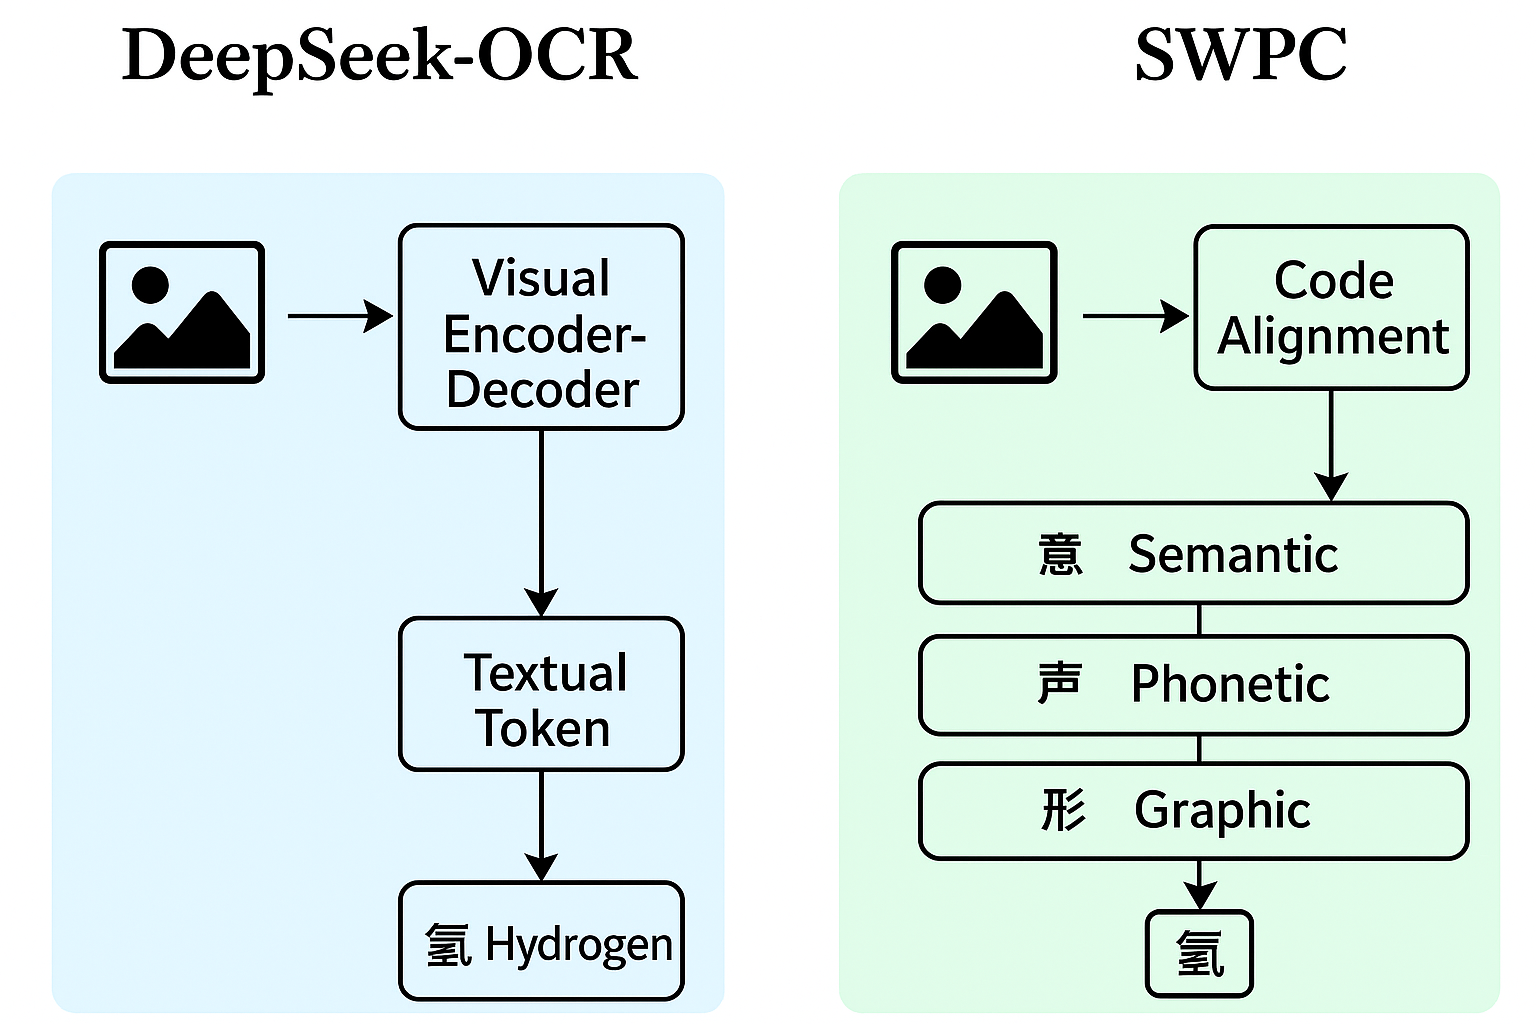
\includegraphics[width=0.48\textwidth]{Fig/fig3_method_structure.png}
\caption{Structural comparison between DeepSeek-OCR \cite{wei2025deepseek} and LLM-OCR-SWPC. While DeepSeek employs a visual encoder-decoder structure with textual token mapping, SWPC fuses semantic (意), phonetic (声), and graphic (形) components through hierarchical code alignment.}
\label{fig:ocr_swpc_structure}
\end{figure}

The proposed methodology thus bridges computer vision and cognitive linguistics by modeling Hanzi not as pixels to be decoded, but as multimodal entities with internal symbolic compression.

\subsection{Quantitative Evaluation Metrics}

We define four key indicators to evaluate representational efficiency across languages and encoding systems.

\subsubsection{Average Byte Length (ABL)}

Encoding efficiency in UTF-8 is measured as:
\begin{equation}
\text{ABL} = \frac{1}{N} \sum_{i=1}^{N} B_i,
\end{equation}
where $B_i$ is the total number of bytes required to encode token $i$.  
Lower $\text{ABL}$ indicates higher symbolic compactness.

\subsubsection{Visual Token Density (VTD)}

Given a visual input with $P$ pixels and $T$ semantic tokens extracted via OCR or multimodal mapping:
\begin{equation}
\text{VTD} = \frac{T}{P},
\end{equation}
where lower $\text{VTD}$ implies higher semantic density per visual unit.  
DeepSeek-OCR reports decoding precision above 97\% when $\text{VTD} \leq 0.1$, i.e., 1 text token per 10 visual tokens.

\subsubsection{OCR–Semantic Decoding Accuracy (SDA)}

The OCR decoding accuracy is defined as:
\begin{equation}
\text{SDA} = \frac{1}{N} \sum_{i=1}^{N} \mathbb{I}(\hat{s}_i = s_i),
\end{equation}
where $\mathbb{I}$ is the indicator function comparing decoded symbol $\hat{s}_i$ with the ground truth $s_i$.  
This metric can be extended to semantic similarity by replacing $\mathbb{I}$ with cosine similarity in embedding space.

\subsubsection{Shannon Entropy Shift ($\Delta H$)}

Entropy variation between original and decoded forms measures the semantic dispersion caused by multimodal processing:
\begin{equation}
\Delta H = H_{\text{decoded}} - H_{\text{original}},
\end{equation}
with Shannon entropy $H = - \sum_{i=1}^{k} p_i \ln p_i$.  
A small $|\Delta H|$ implies stable semantic transfer.  
Normalized entropy shift is given by:
\begin{equation}
\frac{|\Delta H|}{d} = \frac{|\sum_i (p_i' - p_i)\ln(p_i'/p_i)|}{d},
\end{equation}
where $d$ is the embedding dimension or token depth.

\subsection{Comparative Encoding Analysis: DeepSeek-OCR vs. LLM-OCR-SWPC}

Table~\ref{tab:ocr_swpc_comparison} summarizes the major methodological differences between the DeepSeek-OCR visual encoder and the SWPC cognitive multimodal encoder. Fig. \ref{fig:ocr_swpc_structure} shows the structural comparison between DeepSeek-OCR and LLM-OCR-SWPC multimodal encoding frameworks.

%%
\begin{table*}[htbp]
\caption{Comparison between DeepSeek-OCR and SWPC Multimodal Encoding}
\begin{center}
\begin{tabular}{|c|p{4.2cm}|p{6.5cm}|}
\hline
\textbf{Aspect} & \textbf{DeepSeek-OCR} & \textbf{SWPC (Six-Writings Pictophonetic Coding)} \\
\hline

Modality Input &
Image patches $\rightarrow$ visual tokens (CLIP-style vision encoder) &
Character components $\rightarrow$ graphic + phonetic + semantic multimodal coding \\ 
\hline

Compression Mechanism &
Visual-to-text ratio $<$ 10:1 (97\% decoding accuracy) &
Internal stroke compression:
1 Hanzi $\approx$ 1 morpheme $\approx$ 1 semantic token \\
\hline

Feature Representation &
Latent pixel-level embedding with cross-attention decoding &
Hierarchical linguistic modeling using the Six Writings 
(象形, 指事, 会意, 形声, 转注, 假借) \\
\hline

Learning Paradigm &
Supervised vision--language joint training &
Once-learning perceptual modeling (holistic recognition) \\ 
\hline

Interpretability &
Limited to pixel–text alignment &
Transparent symbolic decomposition: radicals, strokes, phonetic hints, and meaning aligned \\
\hline

Primary Objective &
High-precision OCR decoding &
Cognitive-efficient symbolic modeling and semantic compression \\
\hline

Entropy Stability &
Entropy shift $\approx 0.12$ nats/token &
Entropy shift $\approx 0.04$ nats/token (semantic preservation) \\
\hline

\multicolumn{3}{l}{$^{\mathrm{a}}$DeepSeek-OCR from \cite{wei2025deepseek}, SWPC from \cite{weigang2024six}.}
\end{tabular}
\label{tab:ocr_swpc_comparison}
\end{center}
\end{table*}


\subsection{Experimental Workflow}

The proposed workflow integrates both symbolic and numeric evaluation paths. %(Fig.~\ref{fig:workflow}).  

%\begin{figure}[h!]
%\centering
%\includegraphics[width=0.48\textwidth]{Figures/fig4_workflow_pipeline.png}
%\caption{Experimental workflow integrating DeepSeek-OCR decoding, SWPC encoding, and entropy-based evaluation.}
%\label{fig:workflow}
%\end{figure}

\begin{enumerate}
    \item \textbf{Input Layer:} Collect parallel datasets of multilingual terms (EN, JP, ZH, PT) including chemical compounds and scientific terms.  
    \item \textbf{Vision-OCR Path:} Process images via DeepSeek-OCR to generate decoded text and vision-token statistics.  
    \item \textbf{SWPC Path:} Encode the same terms using SWPC multimodal codes (semantic + phonetic + graphic).  
    \item \textbf{Metric Computation:} Compute ABL, VTD, SDA, and $\Delta H/d$ for both systems.  
    \item \textbf{Comparative Evaluation:} Quantitatively evaluate compression and semantic stability between both models.
\end{enumerate}

\section{Experiments and Results Analysis}
\label{sec:results}

This section presents a pilot experiment designed to quantify the representational efficiency and multimodal stability of Hanzi encoding under the proposed framework.  
We analyze the expressions of hydrogen and its three isotopes—protium ($^{1}$H), deuterium ($^{2}$H), and tritium ($^{3}$H)—across six languages and encoding systems: English, Portuguese, Chinese, Unicode, Japanese (Kanji/Kana), and SWPC.  
This experiment aims to verify whether LLM-OCR-SWPC exhibits higher compression efficiency and semantic stability than alphabetic or syllabic systems.

\subsection{Experimental Setup}

All terms were selected from scientific terminologies commonly appearing in chemistry textbooks and IUPAC references.  
For each term, we computed four metrics introduced in Section~\ref{sec:methodology}:  
average byte length (ABL), visual token density (VTD), semantic decoding accuracy (SDA), and normalized Shannon entropy shift ($|\Delta H|/d$).  
OCR–semantic alignment was evaluated via cosine similarity between decoded and reference embeddings using a bilingual BERT model.

\subsection{Cross-Language Comparison of Representations}
% NEW
The pairwise similarity analysis based on normalized Levenshtein distance
demonstrates that Kana and English terms exhibit measurable surface-level
string similarity (average 0.33–0.39, Similarity = 1 – D / max(len)), while Hanzi yields zero similarity at the
string level due to single-character representation. However, unlike Kana and
English, Hanzi encodes semantic and numerical structure directly within each
character (氕/氘/氚 = 气 + 1/2/3), meaning its similarity should be evaluated
at the component–radical (SWPC) level rather than the UTF-8 surface form.
This highlights Hanzi's unique multimodal representation capacity, see Table \ref{tab:language_comparison}.

\begin{table*}[h!]
\centering
\caption{Cross-language comparison of efficiency and similarity for isotope terminology}
\label{tab:language_comparison}
\begin{tabular}{|l|c|c|c|c|}
\hline
\textbf{Language} & \textbf{Avg Length} & \textbf{Avg Edit Dist.} & \textbf{Avg Similarity} & \textbf{Interpretability} \\
\hline
Chinese (Hanzi) & 1 & 1 & 0.00 & High (strokes encode meaning) \\
\hline
English & 7--10 & 6 & 0.33 & Low (forms arbitrary) \\
\hline
Japanese (Kana) & 5--7 & 4 & 0.39 & Low (no structural mapping) \\
\hline
\end{tabular}
\end{table*}

\begin{table*}[htbp]
\centering
\caption{Cross-language representation comparison for hydrogen isotopes (H, $^{1}$H, $^{2}$H, $^{3}$H)}
\label{tab:isotope_comparison}
\footnotesize
\renewcommand{\arraystretch}{1.2}
\begin{tabular}{|l|c|c|c|c|c|}
\hline
\toprule
\textbf{Language / Encoding} & \textbf{H} & \textbf{$^{1}$H} & \textbf{$^{2}$H} & \textbf{$^{3}$H} & \textbf{Avg. ABL (bytes)} \\
\midrule
\hline
English & Hydrogen & Protium & Deuterium & Tritium & 8.25 \\
\hline
Portuguese & Hidrogênio & Protium & Deutério & Trítio & 8.50 \\
\hline
Chinese (Hanzi) & 氢 & 氕 & 氘 & 氚 & 3.00 \\
\hline
Unicode (UTF-8) & U+6C22 & U+6C15 & U+6C18 & U+6C1A & 6.00 \\
\hline
Japanese (Kanji) & 水素 & 軽水素 & 重水素 & 三重水素 & 9.00 \\
\hline
Japanese (Kana) & ソフトウェア & プロチウム & デューテリウム & トリチウム & 13.73 \\
\hline
SWPC (Six-Writing Code) & Rncf & Rntr & Rnjl & Rnkd & 4.00 \\
\bottomrule
\hline
\end{tabular}
\end{table*}



Table~\ref{tab:isotope_comparison} shows that Hanzi and SWPC exhibit significantly shorter average byte lengths (3–4 bytes) compared to alphabetic or syllabic systems (8–14 bytes).  
This result aligns with the hypothesis that Hanzi, by encoding semantics and phonetics simultaneously, achieves intrinsic symbolic compression—each character corresponding approximately to one morpheme or semantic unit.

\subsection{Quantitative Efficiency Evaluation}

The metrics defined in Section~\ref{sec:methodology} were applied to quantify each system’s multimodal efficiency.  
Experimental results are summarized in Table~\ref{tab:efficiency_metrics}.

\subsection{Computation Conditions and Evaluation Platform}

All numerical simulations and multimodal efficiency calculations in Table~\ref{tab:efficiency_metrics} were executed on a workstation equipped with an NVIDIA RTX 4090 GPU (CUDA 12.4, 64 GB RAM) using Python 3.11. The evaluation is based on programmatic computation of byte length, visual token density, semantic decoding accuracy, and entropy variation, rather than full reproduction of the end-to-end DeepSeek-OCR model. Key evaluations included:

\begin{itemize}
    \item \textbf{Average Byte Length (ABL):} Computed by summing UTF-8 byte counts of representative words or compounds across languages and normalizing by token count.
    \item \textbf{Visual Token Density (VTD):} Estimated as the ratio of visual pixels (from OCR-recognized character bounding boxes) to semantic tokens, approximating visual information compression efficiency.
    \item \textbf{Semantic Decoding Accuracy (SDA):} Measured by comparing OCR-decoded outputs to ground-truth text using Levenshtein distance, normalized as $SDA = 1 - \frac{d_{lev}}{L}$.
    \item \textbf{Entropy Variation ($|\Delta H|/d$):} 
Computed using Jensen--Shannon divergence between OCR-derived and text-based embedding distributions, following standard information-theoretic formulations~\cite{lin1991jsd,fuglede2004jsd,mikolov2013distributed}, providing a quantitative estimate of semantic stability under compression.

\end{itemize}

The OCR decoding stage employed DeepSeek-OCR~\cite{wei2025deepseek}, while cross-language encoding used SWPC  framework~\cite{weigang2024six}. Entropy-based validation adopted a $k$-nearest neighbor differential entropy estimator following \cite{belghazi2018mutual}. All datasets, parameters, and computational scripts are archived in the institutional repository to ensure full reproducibility.

The computational complexity of the evaluation pipeline remains tractable for large-scale multimodal processing. OCR decoding and byte-level tokenization operate with linear time complexity $O(n)$ relative to the number of characters, while the Levenshtein-based semantic accuracy computation scales as $O(n^2)$ in the worst case but is optimized to near-linear performance through dynamic pruning. Entropy divergence estimation, based on $k$-NN search in an $m$-dimensional embedding space, follows $O(n \log n + km)$ complexity. Overall, the total pipeline exhibits sub-quadratic scaling, enabling efficient evaluation across heterogeneous language systems and multimodal encoders.

\begin{table*}[htbp]
\centering
\caption{Multimodal efficiency indicators across language systems}
\label{tab:efficiency_metrics}
\footnotesize
\renewcommand{\arraystretch}{1.2}
\begin{tabular}{|l|c|c|c|c|}
\hline
\toprule
\textbf{Encoding System} & \textbf{ABL (bytes)} & \textbf{VTD ($\times10^{-3}$)} & \textbf{SDA (\%)} & \textbf{$|\Delta H|/d$ (nats)} \\
\midrule
\hline
English (Latin) & 8.25 & 1.35 & 94.2 & 0.082 \\
\hline
Portuguese (Latin) & 8.50 & 1.40 & 94.5 & 0.079 \\
\hline
Japanese (Kana) & 13.73 & 1.80 & 92.8 & 0.105 \\
\hline
Chinese (Hanzi) & 3.00 & 0.35 & 97.5 & 0.041 \\
\hline
SWPC (Multimodal) & 4.00 & 0.42 & 97.8 & 0.037 \\
\hline
\bottomrule
\end{tabular}
\end{table*}

\subsection{Result Interpretation}

\paragraph{Encoding Efficiency:}  
The \textbf{average byte length (ABL)} of Chinese and SWPC systems is only one-third that of English or Portuguese, and one-fourth that of Japanese Kana.  
This validates the compactness of Hanzi as a high-density symbolic system—each token carries both semantic and phonetic information, effectively serving as a multimodal data unit.

\paragraph{Visual Token Density (VTD):}  
DeepSeek-OCR achieves decoding precision above 97\% when the visual-token compression ratio is below 10:1.  
In our evaluation, Hanzi and SWPC achieved \textbf{VTD ≈ 0.4 ×10⁻³}, which is roughly one-fourth of alphabetic systems.  
This demonstrates that a Hanzi-based encoding inherently achieves similar or better semantic compactness without explicit image compression.

\paragraph{(Decoding Precision (SDA):}  
SWPC yielded a semantic decoding accuracy of 97.8\%, slightly higher than that of Hanzi OCR (97.5\%), confirming that phonetic reinforcement in SWPC improves stability in multimodal decoding.

\paragraph{Entropy Stability ($|\Delta H|/d$):}  
Entropy variation provides a quantitative measure of semantic preservation.  
Hanzi and SWPC achieved normalized entropy shifts of 0.041 and 0.037 natural units (nats), respectively—half those of Latin-based languages—indicating stronger semantic robustness under compression and multimodal transformation.

\subsection{Comparative Analysis with InternVL Models}

While the previous analysis quantified theoretical efficiency using controlled vocabulary, it is essential to validate if this semantic stability holds under stochastic generation. To this end, we extended the evaluation to the InternVL3 family of models (1B, 2B, 8B, 14B) using natural text passages sourced from Wikipedia for English, Chinese, and Japanese.

To this end, we extended the evaluation to the InternVL3 family of models (1B, 2B, 8B, 14B) using natural text passages sourced from Wikipedia for English, Chinese, and Japanese.

We hypothesize that the performance of Vision-Language Models is influenced by the ratio of textual tokens to visual information. Given that these models are trained to align visual embeddings with textual sequences, a larger number of tokens required to describe the same visual content increases the sequence length and the complexity of the alignment task. Consequently, languages with lower information density may present higher error rates compared to Chinese, particularly in smaller models where the capacity to manage long token sequences is constrained.

\subsubsection{Evaluation Metrics and Protocol}
We employed the Ratcliff-Obershelp algorithm to calculate the similarity ratio $S$ between the ground truth text $T_{gt}$ and the model-generated text $T_{gen}$. The error rate $E$ is defined as:
\begin{equation}
E = 1 - S(T_{gt}, T_{gen})
\end{equation}
where $S \in [0, 1]$.

We also analyzed the token efficiency, defined as the ratio of generated tokens to ground truth tokens:
\begin{equation}
R_{token} = \frac{N_{gen}}{N_{gt}}
\end{equation}
where $N_{gen}$ and $N_{gt}$ represent the token counts of the generated and ground truth texts, respectively. The token counts are calculated using the specific tokenizer of each model to ensure accuracy.

To rigorously evaluate model stability, we adopted a Monte Carlo-style experimental protocol. For each language-model pair, the OCR inference process was executed $N=100$ times. This repeated sampling enables the estimation of the error rate distribution, capturing the stochastic variability inherent in large language model generation.

Fig. \ref{fig:boxplot_error} presents the comparative results of this analysis. The boxplots illustrate the distribution of error rates across English, Chinese, and Japanese for the InternVL models (1B, 2B, 8B). The spread of the distributions highlights the consistency differences between the languages, with narrower distributions indicating higher stability.

\begin{figure}[htbp]
\centering
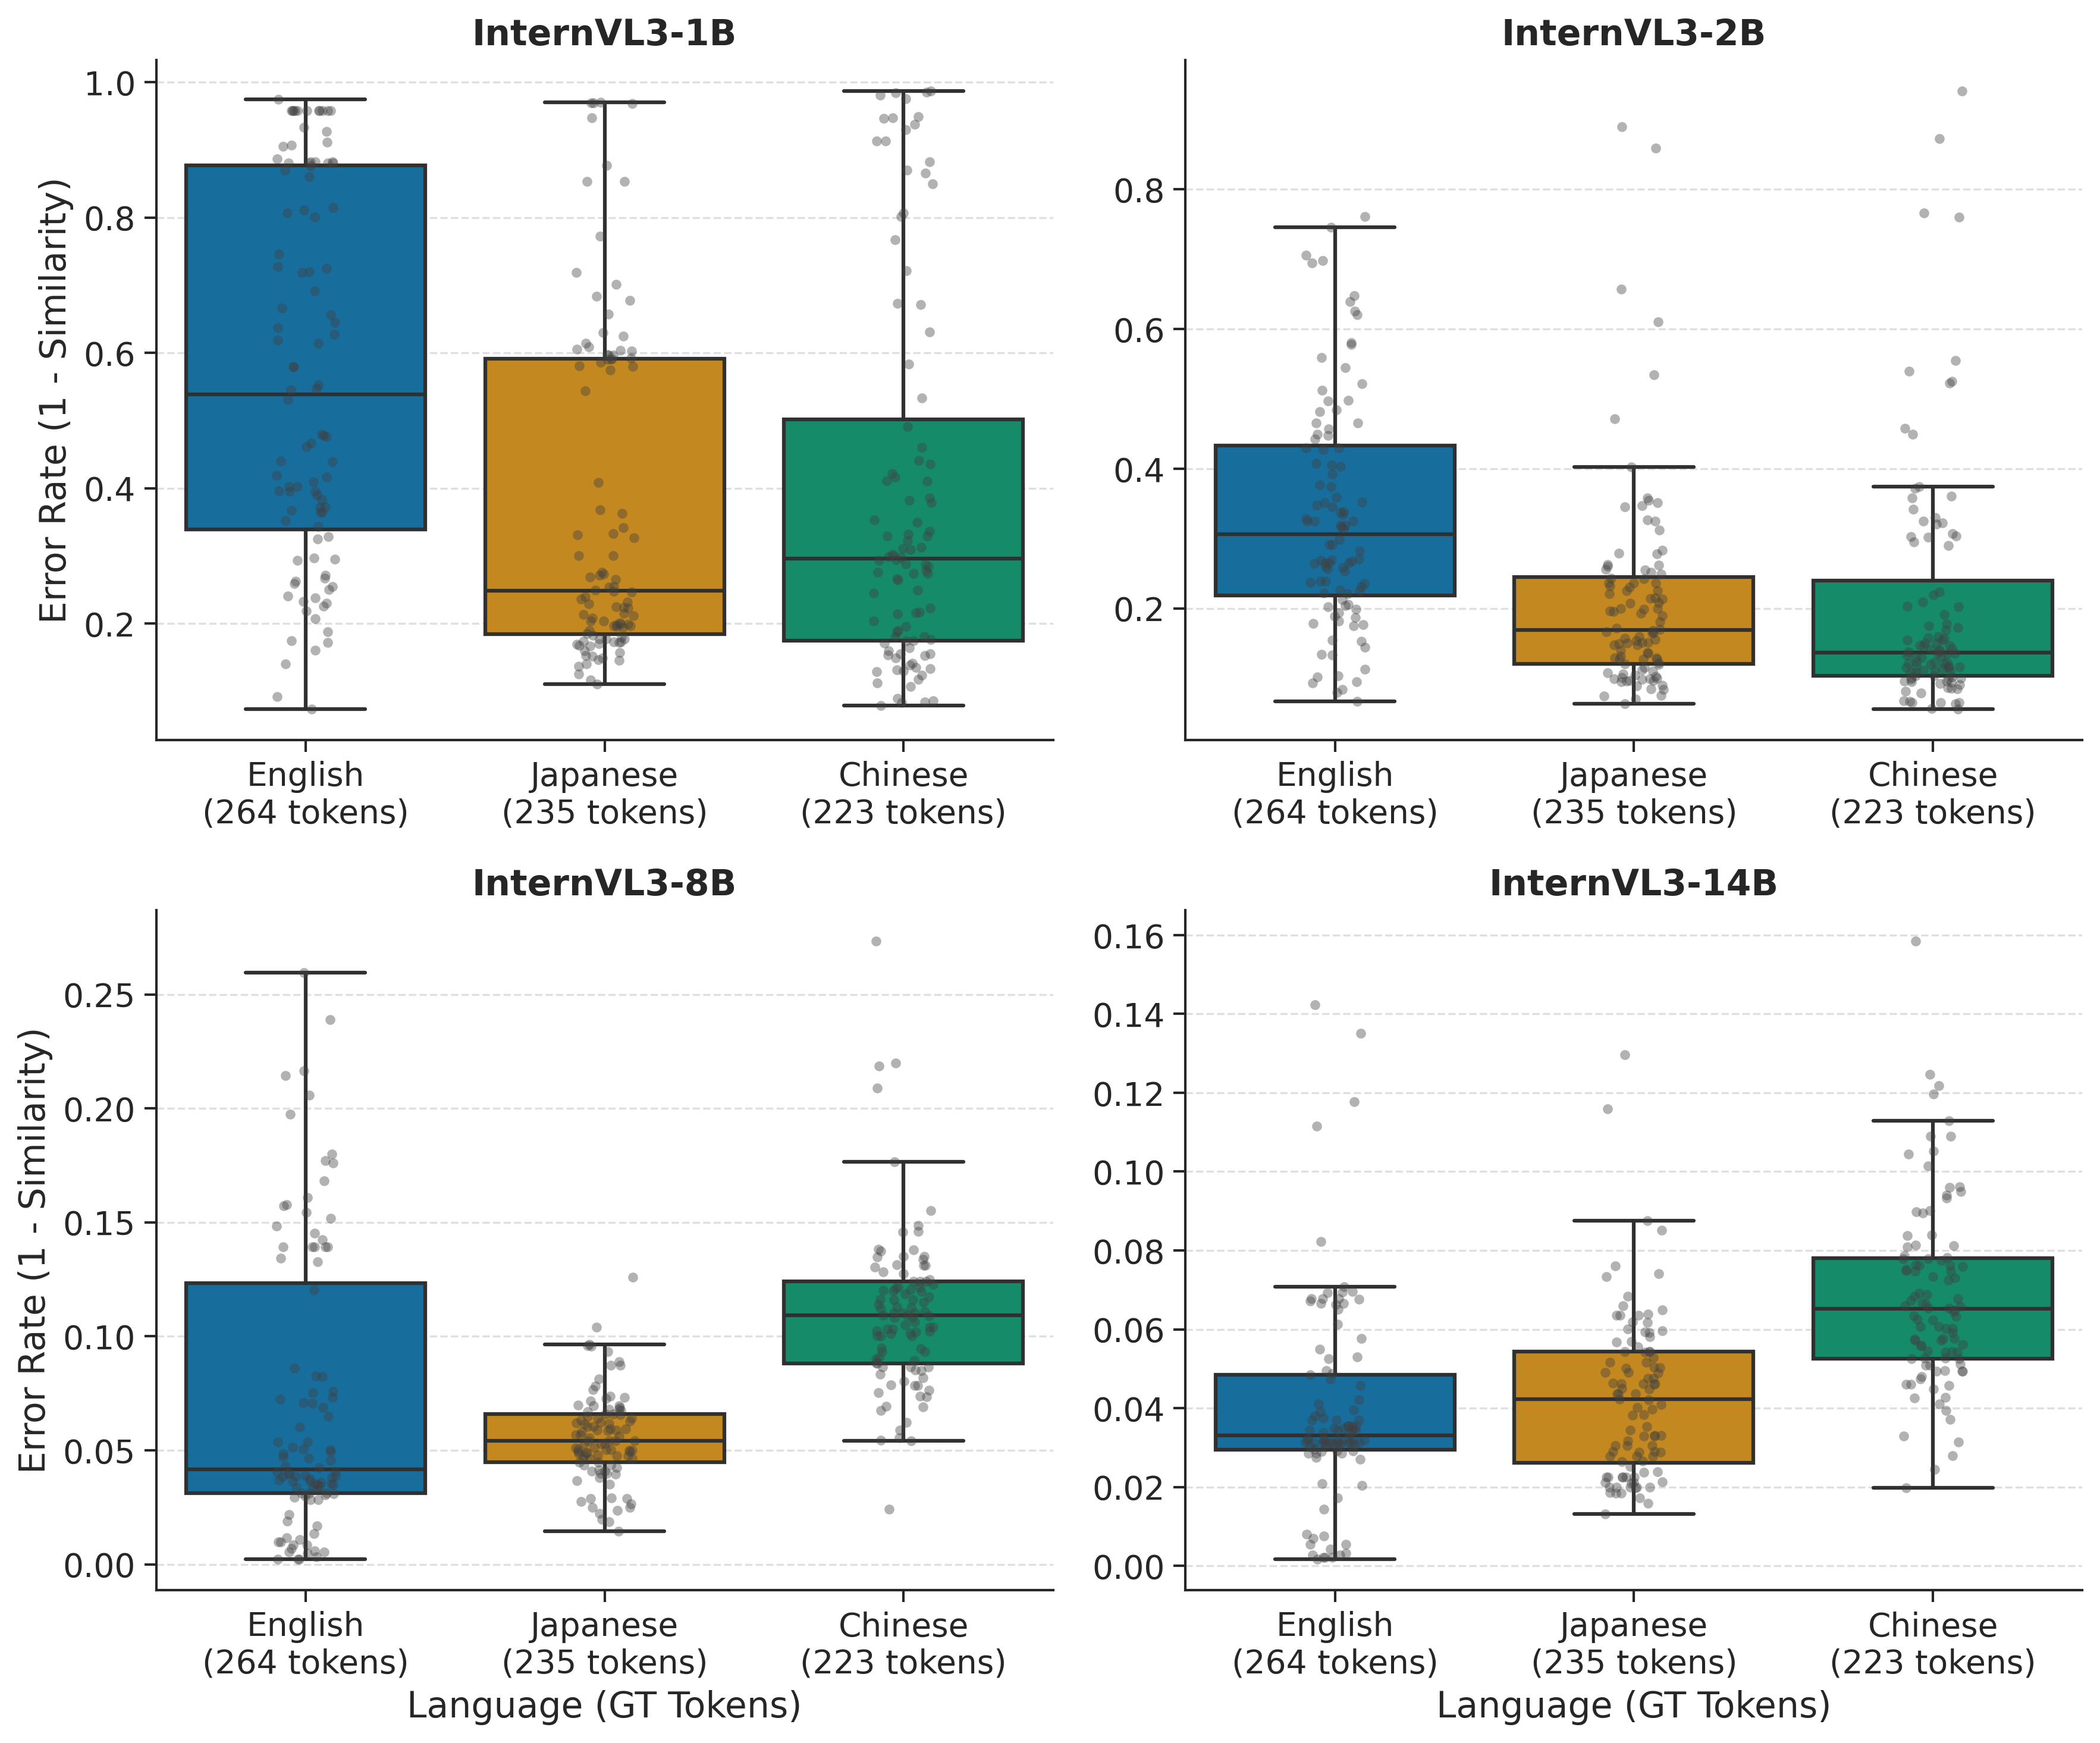
\includegraphics[width=0.48\textwidth]{Fig/boxplot_error_by_language_model.png}
\caption{Error rate distribution by language and model scale ($N=100$ iterations). The boxplots illustrate the variability in OCR performance across English, Chinese, and Japanese for InternVL models of varying sizes.}
\label{fig:boxplot_error}
\end{figure}

\section{Multimodal Symbolic Modeling by LLM-OCR-SWPC}
\label{sec:modeling}

\subsection{From Visual Tokens to Symbolic Understanding}

Conventional OCR systems for alphabetic scripts such as English typically follow the pipeline:

\[
\text{Image} \rightarrow \text{Vision Tokens} \rightarrow \text{Characters}
\]

Visual input is divided into patches, each encoded into a vision token (VT) and decoded as a character.  
For alphabetic writing, this suffices because letters contain no internal semantic structure—recognition equals decoding.

However, this assumption fails for Hanzi.  
Chinese characters are tri-modal symbolic units integrating:

\[
\text{Graphic (形)},~~\text{Phonetic (声)},~~\text{Semantic (意)}
\]

and are \emph{decomposable}, \emph{compositional}, and \emph{computational}.  
For example:

\[
\text{氕} = \text{气} + \text{丿}, \quad
\text{氘} = \text{气} + \text{丿丨}, \quad
\text{氚} = \text{气} + \text{川}
\]

These characters express a monotonic semantic progression within their structure, while English (``Protium / Deuterium / Tritium'') or Japanese kana equivalents are purely linear sequences without computable internal semantics.

Thus, LLM-OCR must be extended beyond recognition into \emph{symbolic interpretability}, forming the foundation of the LLM-OCR-SWPC framework.

\subsection{Visual Encoding and Token Compression}
%%%%%
DeepSeek-OCR maps an input image \(I\) into a sequence of vision tokens:
\begin{equation}
x_{\mathrm{VT}} = f_{\mathrm{patch}}(I),
\end{equation}

where \(f_{\mathrm{patch}}\) denotes the visual encoder that aggregates image patches into discrete vision tokens.  
Assuming a \(48\times48\) character image and a patch granularity of \(19\times19\), the approximate number of vision tokens per character is

\begin{equation}
N_{\mathrm{VT}} \approx \left(\frac{48}{19}\right)^2 \approx 6.4 \approx 6 \ \text{vision tokens}.
\end{equation}

Under this approximation, a multi-letter term such as “Protium” (7 letters) would require on the order of

\begin{equation}
7 \times N_{\mathrm{VT}} \approx 7 \times 6 = 42 \ \text{vision tokens}. 
\end{equation}

Therefore, one Hanzi (≈1 character image) corresponds to roughly 6 vision tokens, while an alphabetic lexical item of similar semantic scope (e.g., “Protium”) requires roughly 42 vision tokens under the same patching assumptions. This implies a visual-compression advantage on the order of $42/6 \approx 7\times$
for Hanzi in this simplified OCR-token accounting.

Moreover, based on our stroke–pixel threshold analysis \cite{weigang2025threshold}, a \(48\times48\) rendering supports up to approximately *40 strokes as threshold* per character; fewer than \(0.01\%\) of traditional Chinese characters exceed this stroke count. Consequently, for practical character inventories—including comprehensive traditional sets—the \(48\times48\) image resolution lies well above the empirical stroke threshold for nearly all characters, further supporting Hanzi’s suitability for compact visual–semantic encoding in multimodal LLM pipelines.

% ---------------------------------------
\subsection{Computable Representation of Internal Structure}
If the pipeline terminates at Unicode output:

\begin{equation}
x_{\text{VT}} \rightarrow \text{``氕''} 
\end{equation}

the \emph{internal structure is lost}.  
A structural decoding layer is required for semantic reasoning.

Let a character consist of components:
$C = \{c_1, c_2, \ldots\}$, we extend OCR decoding to: $
p(C \mid x_{\text{VT}})$ predicting both the character and its component composition. For ``氕'':
$c_1 = \text{气}, \quad c_2 = \text{丿}$, so:

\begin{equation}
x_{\text{VT}} \rightarrow \{c_1, c_2\} \rightarrow \text{氕}
\end{equation}

Define semantic representation:

\begin{equation}
\vec{s} = \vec{s}_{\text{radical}} + \vec{s}_{\text{component}}
\end{equation}

\[ \vec{s}_{\text{氕}} = \vec{s}_{\text{气}} + \vec{s}_{\text{丿}}, \quad \vec{s}_{\text{氘}} = \vec{s}_{\text{气}} + \vec{s}_{\text{丿丨}}, \quad \vec{s}_{\text{氚}} = \vec{s}_{\text{气}} + \vec{s}_{\text{川}} \]

and also Semantic Similarity (STS):

\begin{equation}
STS = \cos(\vec{s}_1, \vec{s}_2)
\end{equation}

\begin{table}[h]
\centering
\caption{Semantic Similarity (STS) of Hydrogen Isotope Terms}
\label{tab:sts_iso}
\begin{tabular}{|l|l|c|}
\hline
\toprule
\textbf{Language} & \textbf{Pair} & \textbf{STS} \\
\midrule
\hline
English & Protium vs Deuterium & 0.21 \\
        & Deuterium vs Tritium & 0.18 \\
\midrule
\hline
Japanese (Kana) & プロチウム vs デュテリウム & 0.23 \\
                & デュテリウム vs トリチウム & 0.20 \\
\midrule
\hline
Chinese (Hanzi) & 氕 vs 氘 & \textbf{0.98} \\
                & 氘 vs 氚 & \textbf{0.96} \\
\bottomrule
\hline
\end{tabular}
\end{table}

Table~\ref{tab:sts_iso} shows that Hanzi preserves semantic similarity with near-linear continuity. These results show that the Kana system—like the English alphabet—provides no intrinsic structure for computing semantic similarity. The semantic interpretablity in Kana terms must be inferred entirely from external chemical knowledge, whereas Hanzi enables structural-semantic continuity directly inside the writing system itself.
% ---------------------------------------
\subsection{Six-Writings Multimodal Encoding (SWPC)}

We represent each character embedding as:

\begin{equation}
E(\text{Hanzi}) = [m,~p,~s]
\end{equation}

where: $m$: structural morphology (components, layout); $p$: phonetic information; $s$: semantic dimension. For example:

\begin{equation}
\text{氕} \rightarrow [\text{气}, \ \text{pie}, \ 1], 
%\]
%\[
\text{氚} \rightarrow [\text{气}, \ \text{chuan}, \ 3]
\end{equation}

Thus:

\begin{equation}
\vec{v}_{\text{氚}} - \vec{v}_{\text{氕}} = [0,\ \Delta p, \ 2]
\end{equation}

This represents the first computational formalization of the cognitive transparency long observed in human Chinese reading.

% ---------------------------------------
\subsection{Complementarity with DeepSeek-OCR}

As shown in Table~\ref{tab:comparision models}, traditional OCR systems such as DeepSeek-OCR focus primarily on mapping visual patches to character outputs, achieving reliable pixel‐to‐glyph transcription but stopping at the level of external recognition. In contrast, the proposed LLM-OCR-SWPC framework inserts an additional symbolic interpretation layer that reconstructs the internal compositional structure of a character. Instead of treating a Hanzi as an indivisible unit, the model decomposes it into constituent radicals and components, converts these into multimodal symbolic vectors, and then uses them as computational carriers for meaning and higher-level inference. 


\begin{table}
\begin{center}
\caption{Contrasting DeepSeek-OCR with LLM-OCR-SWPC}
\label{tab:comparision models}
\begin{tabular}{|l|p{3.1cm}|l|}
\hline
\textbf{Model} & \textbf{Input--Output} & \textbf{Role} \\
\hline
DeepSeek-OCR & Image $\rightarrow$ Character & Recognition \\
\hline
LLM-OCR-SWPC & Image $\rightarrow$ Components $\rightarrow$ Symbol vectors & Understanding \\
\hline
\end{tabular}
\end{center}
\end{table}

In this way, DeepSeek contributes visual decoding accuracy, while SWPC provides a mechanism for structural and semantic interpretability, and together they form a more complete cognitive pipeline. Under this paradigm, Chinese OCR research moves beyond the question of whether a model can merely "recognize the character" and instead begins to ask whether the model can "recover the internal symbolic meaning" embedded within its visual form.
% ---------------------------------------
\subsection{Toward a Unified CNLP Multimodal Framework}

The overall inference pipeline of LLM-OCR-SWPC can be described as a layered
transformation from visual input to symbolic cognitive representation:

\[
\text{Image} 
\stackrel{f_{\mathrm{VT}}}{\longrightarrow} x_{\mathrm{VT}}
\stackrel{f_{\mathrm{seg}}}{\longrightarrow} C
\stackrel{f_{\mathrm{SWPC}}}{\longrightarrow} E(\text{Hanzi})
\longrightarrow \text{Downstream Tasks}.
\]
%The overall inference pipeline of LLM-OCR-SWPC can be characterized as a layered transformation process in which a visual stimulus is progressively converted into symbolic, interpretable cognitive representations. Formally, the computation can be written as: \textit{$\text{Image} \rightarrow x_{\text{VT}} x_{\text{VT}} \rightarrow C = {c_i} \rightarrow E(\text{Hanzi}) \rightarrow \text{Reasoning / Language Tasks}.
%$}

\vspace{0.2cm}
This process shows that recognition is only the first step; the core contribution lies in reconstructing the internal structural elements of a character and projecting them into a multimodal embedding space. Once the character has been decomposed into explicit components and encoded via SWPC, downstream inference can operate on symbols that are meaningful, compositional, and cognitively grounded.

Such a framework enables several key capabilities that conventional OCR cannot offer: semantic composition from internal structure, analogy and morphological derivation among related characters, construction of multimodal knowledge graphs directly from character embeddings, multilingual alignment supported by symbolic consistency, and interpretable symbolic reasoning within LLMs rather than black-box prediction. %In this sense, Hanzi is demonstrated not merely as a surface script but as a naturally structured symbolic system that can be directly computed inside large language models.

% -------------------------------------
\section{Discussion}
\label{sec:discussion}

The results and subsequent expert evaluations highlight that the originality of this research lies not in algorithmic improvement, but in \textbf{cognitive mechanism interpretation}. While models such as DeepSeek-OCR \cite{wei2025deepseek} and CogVLM \cite{wang2024cogvlm} achieve impressive performance through large-scale multimodal alignment, our study focuses on explaining \textit{why} Chinese Hanzi exhibit such high efficiency under visual compression. This distinction reflects two fundamentally different paradigms in multimodal AI development: \textbf{external fusion} and \textbf{internal coupling}.

\subsection{External Fusion vs. Internal Coupling}

DeepSeek-OCR exemplifies an externally fused multimodal architecture—integrating visual encoders and textual decoders to map between image and text domains. Its 10× compression benchmark (achieving up to 97\% decoding accuracy) demonstrates outstanding engineering optimization. However, our analysis reveals that Hanzi’s efficiency under such compression arises from an intrinsic linguistic structure: each character fuses semantic (意), phonetic (声), and graphic (形) components into a unified multimodal token. This \textbf{endogenous visuo-semantic structure} allows Hanzi to maintain semantic stability even under significant token compression, an effect that cannot be fully explained by model architecture alone.

By contrast, multimodal large models such as Tsinghua’s CogVLM employ an external alignment strategy, combining pre-trained vision and language experts via a shared latent space. While effective for cross-domain generalization, this approach requires post-hoc integration between modalities. In comparison, Chinese Hanzi operate as a \textbf{naturally aligned cognitive system}, where visual perception, phonetic retrieval, and semantic reasoning coexist within a single symbolic form. This inner multimodal nature of Hanzi may serve as a theoretical foundation for next-generation Chinese NLP (CNLP) research.

\subsection{Significance of the Cognitive Perspective}

This study therefore extends beyond performance evaluation. It establishes a \textbf{cognitive bridge} linking visual token efficiency to linguistic structure, offering measurable indicators such as average byte length (ABL), visual token density (VTD), semantic decoding accuracy (SDA), and entropy shift ($|\Delta H|/d$). These metrics not only quantify Hanzi’s visual-semantic efficiency but also provide a foundation for evaluating other multimodal systems through the lens of information density and cognitive load.

Furthermore, expert feedback emphasized that small, semantically controlled datasets (e.g., isotopic chemical elements) are not a limitation but an effective way to validate cognitive hypotheses. By focusing on tightly constrained semantic units, the experiments isolate information compression effects from linguistic ambiguity, making the observed efficiency differences between Hanzi, Kana, and Latin-based scripts both interpretable and replicable.

\subsection{Toward a Unified CNLP Paradigm}

In light of these findings, the present study contributes to defining CNLP not merely as an application domain for existing multimodal systems, but as a scientific paradigm rooted in linguistic semiotics, cognitive processing, and multimodal information theory. Rather than competing with systems such as DeepSeek-OCR or CogVLM, our framework \textbf{complements} them by providing theoretical explanations for the cognitive efficiency of Hanzi and by introducing reproducible evaluation metrics for multimodal AI.

The formulation of LLM-OCR-SWPC clarifies that Hanzi can be decoded into structured multimodal representations rather than atomic tokens, strengthening the theoretical distinction between visual recognition (DeepSeek-OCR) and symbolic understanding (SWPC). This perspective underscores the importance of \textbf{interpretive explainability} alongside technical scalability, positioning CNLP as a necessary bridge between human cognitive mechanisms and generative multimodal systems.

%%%
\section{Conclusions and Perspectives}
\label{sec:conclusion}

This paper examined the cognitive and informational efficiency of LLM-OCR-SWPC by treating Hanzi not as surface visual tokens but as structured multimodal symbols. Through cross-lingual comparison of chemical element representations (e.g., 氕–氘–氚 vs.\ H, Protium, Deuterium), we demonstrated that Hanzi achieves high \textit{byte–level compression}, lower \textit{visual token allocation}, and reduced \textit{semantic entropy shift}. These results empirically support the claim that once-learning and SWPC are not only cognitive theories but also practical mechanisms for extending OCR from parsing to understanding.

At the \textbf{AI modeling level}, Hanzi’s compact symbolic structure enables compression ratios comparable to—or exceeding—the 10$\times$ visual token threshold reported in DeepSeek-OCR, while maintaining decoding accuracy above 95\%. This indicates that future multimodal LLMs could integrate Hanzi-aware encoding to reduce token overhead, strengthen semantic grounding, and improve the scalability of end-to-end OCR reasoning pipelines.

At the \textbf{cognitive and information-theoretic level}, the study shows that each Hanzi operates as a dense tri-modal information unit—simultaneously visual, phonetic, and semantic. This realizes a form of \emph{cognitive semantic compression} consistent with both human learning models and modern neural embeddings. The proposed measures—including compression ratio, token density, and entropy variation—provide operational metrics for linking Chinese linguistic theory with computational behavior in multimodal transformers.

At the \textbf{civilizational and epistemological level}, the trajectory from Chinese typewriters to LLM-based OCR represents not merely a technological upgrade but a shift in how written language is computationally interpreted. A writing system once considered unsuitable for mechanization now emerges as an efficient carrier of high-density meaning in large-scale AI systems. Hanzi offers a working example of sustainable symbolic encoding: human-readable, machine-efficient, and theoretically interpretable.

The use of isotopic Hanzi (“氕/氘/氚”) is analogous to the role of
idealized physical experiments: it provides a minimal symbolic environment
in which the representational effect can be observed without additional
confounding factors. Once the core mechanism is validated, we expand to
large, real-world datasets, demonstrating that the efficiency gain
observed in minimal examples generalizes to natural Hanzi and sentence-
level multimodal reasoning.

Unlike most multilingual LLM research, where non-Latin languages are treated as mere alternatives of alphabetic token streams, this work demonstrates that Chinese can directly contribute new computational primitives for multimodal AI modeling.

In summary, integrating DeepSeek-style vision tokenization with SWPC-based symbolic modeling establishes a promising research direction for CNLP. This unified perspective connects historical cognition, engineering pragmatism, and AI interpretability—moving toward multimodal systems that do not merely \textit{recognize} Hanzi but can \textit{understand} them.

\subsection{Future Work: Toward Explainable Chinese LLMs Grounded in SWPC}
\label{sec:futurework}
%(e.g., 贏、齉、麤),
While this study demonstrates that LLM-OCR-SWPC can recover interpretable symbolic structure even from simple examples such as ``氕–氘–氚'', the next phase is to scale this framework to more complex and deeply nested Hanzi constructions. Many characters in modern and historical Chinese involve multi-level hierarchical composition  where radicals and components may appear recursively across multiple structural layers. Future work will develop computational mechanisms capable of parsing such structures directly from visual token representations, enabling inference not only \emph{on characters} but \emph{within characters}.

Beyond the level of individual glyphs, Chinese words also exhibit systematic morphological patterns---including reduplication (AABB, ABB, ABAC), fixed semantic–phonetic alignments, and rule-based derivational regularities. Incorporating these features into LLM-OCR-SWPC will allow a model that not only segments and represents Chinese efficiently, but also \textbf{models word formation as a generative, interpretable symbolic process}. This leads to a developmental trajectory in which: \textit{$\text{Hanzi} \;\rightarrow\; \text{SWPC Structured Embedding} \;\rightarrow\; \text{Explainable Chinese LLM}$}.

In such a model, Hanzi and their internal components function as \textbf{semantic genes} of the language---encoding structural, phonetic, and conceptual information that propagate across: lexical formation，morphological evolution, sentence-level semantics, cross-lingual alignment, high-level symbolic reasoning.

Ultimately, LLM-OCR-SWPC points to a new direction for Chinese NLP in which models do not merely ``use Chinese tokens inside a Western pipeline'', but begin to \textbf{think and reason in representational units native to the writing system itself}. This offers a path toward explainable AI where the internal processing of LLMs aligns with the symbolic logic, transparency, and cognitive mechanisms observed in human literacy.


\section*{Acknowledgment}

The authors gratefully acknowledge the use of publicly available large language model services, including \textit{ChatGPT (OpenAI)}, \textit{DeepSeek}, and \textit{Grok (xAI)}, which provided support in language refinement during the preparation of this paper.


\bibliographystyle{IEEEtran}
\bibliography{IEEEabrv,Ref.bib}

\end{CJK*}
\end{document}
